%\documentclass[12pt,preprint]{aastex}
\documentclass[apjl]{emulateapj}

\pdfoutput=1

\usepackage{comment}
\usepackage{ifthen}
\usepackage{amsmath}
\usepackage{amsfonts}
\usepackage{amssymb}
\usepackage{multirow}
\usepackage{wasysym}
\usepackage{subfigure}
\usepackage{epsfig}
\usepackage{color}
\definecolor{linkcolor}{rgb}{0,0,0.5}
\usepackage[%
	colorlinks=true,	% false: boxed links; true: colored links
	pdfpagelabels=true,
	hypertexnames=true,
	plainpages=false,
	naturalnames=true,
%	bookmarks=true,         % show bookmarks bar?
%	unicode=false,          % non-Latin characters in Acrobat’s bookmarks
%	pdftoolbar=true,        % show Acrobat’s toolbar?
%	pdfmenubar=true,        % show Acrobat’s menu?
%	pdffitwindow=false,     % window fit to page when opened
%	pdfstartview={FitH},    % fits the width of the page to the window
	pdftitle={Priors for Orbital Eccentricity},    % title
	pdfauthor={David M. Kipping},     % author
%	pdfsubject={Subject},   % subject of the document
%	pdfcreator={Creator},   % creator of the document
%	pdfproducer={Producer}, % producer of the document
%	pdfkeywords={keyword1} {key2} {key3}, % list of keywords
%	pdfnewwindow=true,      % links in new window
	urlcolor=linkcolor,     % color of external links
	linkcolor=linkcolor,    % color of internal links (change box color with linkbordercolor)
	citecolor=linkcolor,    % color of links to bibliography
	filecolor=linkcolor,    % color of file links
        ]{hyperref}
%

% #############################################################################
% Specific latex definitions for this paper

\newcommand{\logg}{$\log g$}
\newcommand{\rhostar}{$\rho_{\star}$}
\newcommand{\Teff}{$T_{\mathrm{eff}}$}
\newcommand{\FeH}{[Fe/H]}
\newcommand{\Kepler}{\textit{Kepler}}

%% #############################################################################

%% VARIABLE DEFINITIONS
%%
\newboolean{emulateapj}
\setboolean{emulateapj}{true}

\newboolean{astroph}
\setboolean{astroph}{true}

\newboolean{png}
\setboolean{png}{false}

\newboolean{color}
\setboolean{color}{true}

%% ############################################################################

\shortauthors{Angus \& Kipping}
\shorttitle{Probabilistic Inference of Stellar Parameters}
\ifthenelse{\boolean{emulateapj}}{
    \newcommand{\titledag}{$\dagger$}
}{
    \newcommand{\titledag}{\dagger}
}
\def\mathbi#1{\textbf{\em #1}}

\begin{document}

%% Titlepage
\title {Probabilistic Inference of Basic Stellar Parameters:\\
Application to Flickering Stars %to Surface Gravity and Mean Density
\altaffilmark{\titledag}}

%% Authors
\author{
	{\bf	Ruth~Angus\altaffilmark{1,2},
		David.~M.~Kipping\altaffilmark{2,3},
	}
}

\altaffiltext{1}{Dept. of Physics, University of Oxford, UK; email:
		 ruth.angus@astro.ox.ac.uk}

\altaffiltext{2}{Harvard-Smithsonian Center for Astrophysics,
		Cambridge, MA 02138, USA; email: dkipping@cfa.harvard.edu}

\altaffiltext{3}{Department of Astronomy, Columbia University, 550 W 120th St.,
                 New York, NY 10027, US}

\altaffiltext{$\dagger$}{
%%
Based on archival data of the \Kepler\ telescope.
}


%% EOF authors

% #####################################################################
%% abstract
\begin{abstract}

% aims
The relations between observable stellar parameters are usually assumed to be
deterministic, that is, given an infinitely precise measurement of independant
variable, `$x$', and some model, the value of dependant variable, `y' can be
known exactly.
In practise this assumption is rarely valid and intrinsic stochasticity means
that two stars with exactly the same `$x$', will have slightly different
`$y$'s.
% methods
The relation between short-timescale brightness fluctuations (flicker) of
stars and both surface gravity \citep{bastien:2013} and stellar density
\citep{kipping:2014} are two such stochastic relations that have, until now,
been treated as deterministic ones.
We recalibrate these relations in a probabilistic framework, using
Hierarchical Bayesian Modelling (HBM) to constrain the instrinsic scatter in
the relations.
% Our treatment also fully accounts for the observational uncertainties on all
% variables.
% results
We find evidence for additional scatter in the relationships, particularly in
the relation between flicker and surface gravity, that cannot be accounted for
by the observational uncertainties alone.
The scatter in surface gravity increases with decreasing flicker, i.e. there
is greater scatter for subgiants than for dwarfs, suggesting that using flicker
as a proxy for surface gravity is just as (if not more) valid for dwarf stars,
despite the fact that the observational uncertainties tend to be larger for
these stars.

\end{abstract}

% #####################################################################
%% keywords
\keywords{
%%
	stars: fundamental parameters --- techniques: photometric ---
        methods: statistical
%%
}

%% EOF keywords
%% EOF titlepage

% #####################################################################
%% Introduction
\section{INTRODUCTION}
\label{sec:intro}

%% INTRODUCTION
%%

Accurate stellar characterization plays a vital role for many active research
fields within astronomy. For example, stellar populations, galactic
archaeology, the study of binary stars, asteroseismology and exoplanet studies
all rely on inferences of basic stellar parameters to varying degrees.
Empirically-derived and reliable estimates are of particular value, increasing
our confidence in the end-product results built upon these inputs.

Basic stellar parameters, such as effective temperature and surface gravity,
can be inferred using one (or more) of several types of observations, such as
spectroscopy, photometry, interferometry, etc. This inference can be performed
by invoking theoretical models or by building an empirical calibration
library.
For example, an observed stellar spectrum could be matched against a library of
theoretical spectra generated using stellar atmosphere models, or, against a
library of observed spectra of ``standard stars'', serving as calibrators.
%Fundamental stellar parameters, such as mass and radius, which cannot be
%directly inferred from the available observations can often be inferred by
%invoking theoretical stellar models, e.g. fitting model isochrones to
%spectroscopic measurements.
Regardless of the approach, be it theoretical or empirical, the methods used
for the inference of stellar parameters are traditionally ``deterministic''.
In this context, a deterministic model can be loosely described as one where
a particular observational input always returns a single-valued output for a
parameter of interest, i.e. nature itself has no variance and the underlying
model is considered to be a perfect description of reality.

An alternative approach for inferring model parameters is to allow
relationships between observables to be stochastic.
Unlike the deterministic case, a single observational input is intepreted to
be caused by a range of possible model parameters, described by a probability
distribution.
This statement is true even in the case of a perfect observation of infinite
signal-to-noise, since the underlying model itself comes with uncertainty.
In recent years, there has been a shift towards such methods in several areas
of astronomy, particularly within the exoplanet community.
For example, \citet{wolfgang:2015} considered that the mass-radius
relationship of exoplanets is stochastic, since a particular sized planet
could be have a range of planet masses due to unmodeled variances in
compositions, environment and other complications.
These recent demonstrations in exoplanetary science have prompted us to
consider the need for treating the parent stars in the same probabilistic
framework, with potential applications spanning many fields of astronomy.

The demand for probilistic stellar parameters is not only motivated by the fact
that probability distributions are far more representative of our `beliefs'
about astrophysical parameters, it also has a practical purpose.
When using data published in the astronomical literature to, for example, infer
relationships between observed parameters, that inference can be performed as
the final stage in a hierarchical treatment
\citep[see, e.g.][]{foreman-mackey:2014}.
This is useful if, for example, one wants to account for multi-dimensional
uncertainties by marginalizing over the `true' parameter values upon which the
noisy observations are conditioned.
This point is discussed further in \textsection\ref{sec:HBM}.

%A number of recent exoplanet studies have used Hierarchical Bayesian Modeling
%(HBM) to model the dispersion, or intrinsic scatter in relations between
%astrophysical properties.
%For example, \citep{wolfgang:2015} use HBM to recalibrate the mass-radius
%relation for sub-Neptunes and infer the level of astrophysical dispersion

% RA text...

One of the more recent tools developed to characterize stars is known as
``flicker'' \citep{bastien:2013}.
Flicker is a proxy for the scatter on an 8-hour timescale (denoted as $F_8$)
in a broad visible bandpass time series photometric light curve, such as that
from \textit{Kepler} or the upcoming TESS mission. A more detailed account of
the proceedure to calculate flicker is described in \citet{bastien:2013}. As
shown in \citet{bastien:2013}, flicker displays a remarkable correlation to
the asteroseismically determined parent star surface gravities (\logg).
Turning this around, the observation implies that flicker can be used to
blindly infer surface gravities at the level of $\sim0.1$\,dex, an attractive
proposition given the wealth of photometric light curves available through the
array of exoplanet transit missions flying and scheduled to launch.

\citet{cranmer:2014} demonstrated that models of stellar surface granulation
indeed reproduce a flicker effect in close agreement with that observed by
\citet{bastien:2013}, providing a physically-plausible explanation.
Since surface gravity is highly correlated with mean stellar density (\rhostar)
on evolutionary tracks, \citet{kipping:2014} showed that flicker can be also
be used to infer \rhostar, which is more useful for exoplanet transit analysis
\citep{seager:2003}.

Whether one calibrates flicker to \logg\ or \rhostar, there are several aspects
of the problem which are attractive for our purposes of a simple demonstration
of probabilistic inference of stellar parameters.
Firstly, in log-log space the relationship is very simple, appearing to be
linear \citep{kipping:2014}.
Secondly, there is a sufficiently large number of points in the sample (439
stars) to constrain a population-based model.
Thirdly, there is significant excess scatter around the best-fitting relation
implying that a deterministic model is inadequate.
This is not surprising given that granulation is a complex and messy process
for which one should not expect any parametric model to provide a perfect
description.
Fourthly, the physical processes that produce surface granulation, of which
flicker is an observational tracer, may be more or less noisy for different
types of stars.
We will test whether flicker has greater predictive power in certain regions
of parameter space; i.e. is flicker significantly more informative for
subgiants than for dwarfs?
For these reasons, we identify the calibration of
flicker to \logg\ and \rhostar\ as a well-posed problem to first demonstrate
probabilistic inference in the arena of stellar characterization.

\section{PROBABILISTIC CALIBRATION}
\label{sec:HBM}

%% HBM
%%

\subsection{Calibration Data}

For our calibration data, we used a sample of \Kepler\ stars with
both asteroseismic and flicker measurements available. \citet{chaplin:2014}
report asteroseismic \rhostar\ estimates (and the associated uncertainties) for
518 \Kepler\ stars. The authors report three different sets of results,
depending on the choice of \Teff\ and \FeH, and in this work we elected to use
values reported in their Table 6 over Table 5, and Table 5 over Table 4. We
additionally used the 71 additional planet hosting stars with asteroseismology
reported in \citet{huber:2013} but not reported in \citet{chaplin:2014}. Values
for flicker and ``range'' were taken from \citet{kipping:2014}, based upon the
methods described in \citet{bastien:2013}. Following \citet{kipping:2014} and
for reasons described there-in, we only include targets in our calibration for
which:

\begin{itemize}
\item[{\tiny$\blacksquare$}] Range (defined in \citealt{bastien:2013})
$<1$\,ppt
\item[{\tiny$\blacksquare$}] $4500<T_{\mathrm{eff}}<6500$\,K
\item[{\tiny$\blacksquare$}] $K_P<14$
\item[{\tiny$\blacksquare$}] $1.2 < \log_{10}$($F_8$\,[ppm])$< 2.2$
\end{itemize}

We use the same sample for our calibration of \logg, except that we exclude the
\citet{huber:2013} data, since these authors do not provide estimates of
\logg\footnote{Whilst we could compute \logg\ ourselves from the reported
masses and radii, this could only be done under the incorrect assumption of
zero covariance between $M_{\star}$ and $R_{\star}$.}.

\subsection{Hierarchical Bayesian Model}

We model the stochastic relationship between $F_8$ and \logg\ or \rhostar,
accounting for the fact that there exists some intrinsic scatter in
the dependent variable, and including the heteroskedastic uncertainties on both
the dependent and independent variables.
There are two excellent reasons for modelling the relation stochastically;
firstly, if the intrinsic scatter is ignored and the relation between
variables is assumed to be deterministic, those data points with smaller
measurement uncertainties may have an unrepresentative greater weighting
during the fitting process \citep{hogg:2010b}.
Secondly, we are interested in producing probability distributions over stellar
densities and surface gravities, as opposed to point estimates, and propagating
these probability distributions through to subsequent analyses.
Several recent studies have required posterior Probability Distribution
Function (PDF) samples, in order to conduct their (hierarchical)
analyses \citep[e.g.][]{foreman-mackey:2014, rogers:2015, angus:2015}.

Including observational uncertainties on the independent variable within our
analysis is also important, because ordinary least squares regression methods
performed on data with two-dimensional uncertainties will result in a slope
that is biased towards zero
\citep[e.g.][]{fuller:1987, fox:1997}.
For a demonstration of the affects of neglecting intrinsic scatter and
two-dimensional uncertainties, see \citet{kelly:2007}.

We write the two models describing the relationship between $F_8$, \logg\ and
\rhostar\ as
\begin{equation}
	\log_{10}(\rho_\star) \sim \mathcal{N} \left(\mu = \alpha + \beta
	\log_{10}(F_8), \sigma = \sqrt{\sigma_{\rho}^2 + \gamma F_8}\right),
\end{equation}
\label{eq:rho}
and
\begin{equation}
	\log_{10}(g) \sim \mathcal{N}\left(\mu = \delta + \epsilon \log_{10}(F_8),
	\sigma = \sqrt{\sigma_g^2 + \zeta F_8}\right).
\end{equation}
\label{eq:logg}
The free parameters of the two models are $\alpha$, $\beta$, $\gamma$
$\sigma_{\rho}$, $\delta$, $\epsilon$, $\zeta$ and $\sigma_g$.
These relations are Gaussian distributions with means
given by the equation of a straight line, and standard deviations which
describe the intrinsic scatter about the mean as a function of flicker.

In order to account for the two-dimensional observational uncertainties in
this data set, we marginalize over the latent, `true' values of $F_8$,
\rhostar\ and \logg\ using the importance sampling method of
\citep{hogg:2010}\footnote{Note that while the pseudo-marginal MCMC method of
\citep{andrieu:2009} provides a truly unbiased estimate of the marginalized
likelhood, we expect any bias introduced by the importance sampling method to
be negligable.}.
In what follows we give an overview of this procedure, but encourage the
reader to refer back  to this original reference for a more detailed
description of the mathematics.
The observed values of the variables; $F_8$, \rhostar\ and \logg\ can be
thought of as a single `draw' from an underlying (assumed Gaussian)
probability
In what follows we give an overview of the importance sampling procedure, but
encourage the reader to refer back to the original reference for a more
detailed description of the mathematics.
The observed values of the variables; $F_8$, \rhostar\ and \logg\ can be
thought of as a single `draw' from an underlying (assumed Gaussian)
probability distribution, with mean equal to the `true' value---the value that
would have been observed, given infinitely high signal-to-noise---and standard
deviation equal to the observational uncertainty.
We compute the likelihood of the data given the model, marginalized over the
true values, using importance sampling.
We sample from the posterior PDFs of the true values of the variables,
conditioned on the observed values, and compute the likelihood of each of those
samples.
% These posterior PDFs could be produced by the astronomers who provide the
% catalog.
% If posterior samples are made available, they can be used in this stage of
% the inference.
% In the event that they are not provided however, they can be generated.
% For example, the $log(g)$ values used here are point estimates of the
% posterior PDFs of $log(g)$, produced by \citet{chaplin:2014} using
% {\it Kepler} light curves and stellar models.
We would use the posterior samples generated in previous model fitting process
if they were available, however generating new samples is an acceptable
approximation provided the posteriors are Gaussian and the priors used by the
previous fitters were uninformative.
Such an approximation will not be necessary for those studies using \rhostar\
or \logg\ calculated using the newly-calibrated relations presented here,
since we have published our posterior samples.
After producing new posterior PDF samples we then add up the individual
log-likelihoods of each sample to compute the total marginalized likelihood
for a star.
The marginalized likelihood of the whole dataset is then computed as the sum
of the log-likelihoods of each star.
The importance sampling method allows us to approximate the integral over the
latent variables.
% We used flat priors for all except the $\sigma$ parameters, for which we used
% priors which were flat in log-space.
We used uniform priors over all our parameters:
\begin{eqnarray}
	&	\alpha, \beta, \delta, \epsilon
	\sim U(-10:10) \\ \nonumber
 	&	\sigma_{rho}, \gamma, \sigma_g, \zeta  \sim U(-100:100).
\end{eqnarray}
\label{eq:priors}

We also performed this inference using an alternative, analytic form of the
marginal likelihood, which accounts for 2-D uncertainties but does not allow
the intrinsic scatter to be a function of the dependent or independent
variables.
For the relation between flicker and \rhostar, this likelihood function can be
written as
\begin{eqnarray}
	& p(\rho_*| F_8, \alpha, \beta, \sigma_{\rho}) =  \\ \nonumber
						      & \exp \left[-\frac{1}{2}
		\sum_{n=1}^N \frac{[F_{8n}-(\alpha + \beta \rho_{*n})]^2}
	{\left[\beta \sigma_{F8, n}^2 + (\sigma_{\rho *, n}
	+ \sigma_{\rho})^2\right]}\right]
	\\ \nonumber
	& + \beta^2 \sigma_{F8, n}^2 + (\sigma_{\rho *, n} + \sigma_{\rho})^2,
\end{eqnarray}
\label{eq:likelihood}
and similarly for \logg.
The parameter values found using this simple likelihood function are included
in table \ref{tab:results}.
% The analytic likelihood function, equation \ref{eq:likelihood} is suitable for
% cases where the intrinsic scatter is not a function of $x$ or $y$.
Figures \ref{fig:rhostar} and \ref{fig:logg} show the data with the best-fit
models.
The shaded regions show the 1 and 2$\sigma$ confidence interval which are
representative of the intrinsic scatter in the relations.
% Given a measurement of flicker, the predictive probability distribution of
% \logg and \rhostar will be a Gaussian distribution

%%% rhostar plot
\begin{figure}
\begin{center}
% \includegraphics[width=8.4cm,angle=0,clip=true]{../figs/rho_vs_flicker.pdf}
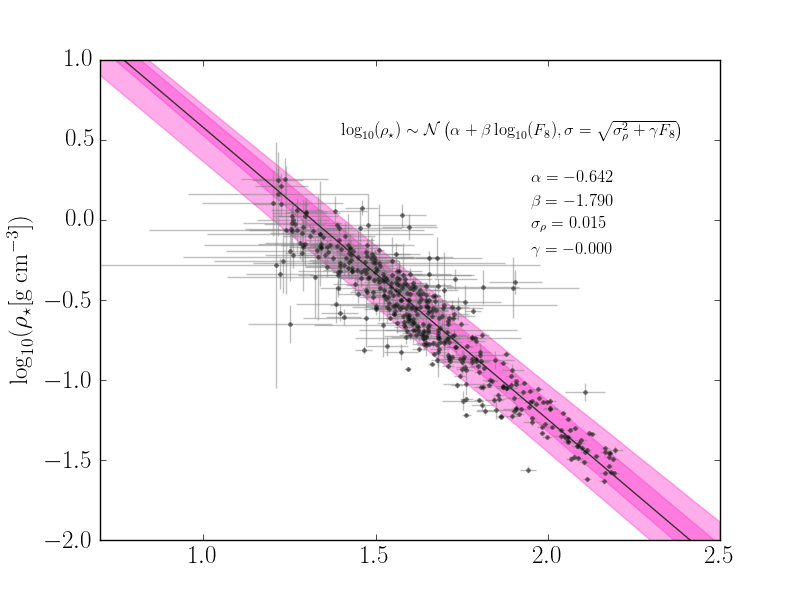
\includegraphics[width=8.4cm,angle=0,clip=true]{new_rho.pdf}
\caption{
Stellar density vs. flicker.
This figure shows the model, conditioned on the data.
The solid black line shows the highest-likelihood sample, and the pink shaded
regions show the 1 and 2$\sigma$ confidence intervals.}
\label{fig:rhostar}
\end{center}
\end{figure}

%%% logg plot
\begin{figure}
\begin{center}
% \includegraphics[width=8.4cm,angle=0,clip=true]{../figs/logg_vs_flicker.pdf}
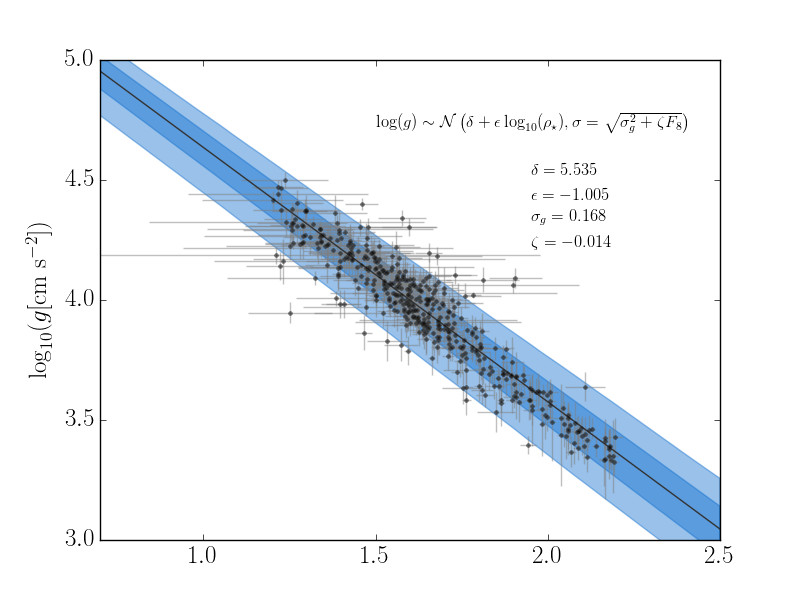
\includegraphics[width=8.4cm,angle=0,clip=true]{new_logg.pdf}
\caption{
$\log(g)$ vs. flicker.
As in \ref{fig:rhostar} this figure shows the model, conditioned on the data.
The solid black line shows the highest-likelihood sample, and the blue shaded
regions show the 1 and 2$\sigma$ confidence intervals.}
\label{fig:logg}
\end{center}
\end{figure}

\begin{table}
\caption{Highest-likelihood parameter values with 16th and 84th
	percentile uncertainties.}
\begin{tabular}{lccc}
\hline\hline
Parameter & highest-likelihood value & simple model result \\
    \hline
$\alpha$ &    2.358$_{-0.04}^{+0.08}$ &       2.191$_{-0.05}^{+0.05}$  \\
$\beta$ &    -1.79$_{-0.03}^{+0.04}$ &        -1.724$_{-0.03}^{+0.03}$ \\
$\sigma_{rho}$ &    0.015$_{-0.04}^{+0.08}$ &   0.085$_{-0.05}^{+0.05}$  \\
$\gamma$ &    -0.0$_{-0.04}^{+0.08}$ & \\
$\delta$ &    5.535$_{-0.07}^{+0.07}$ &      5.739$_{-0.03}^{+0.03}$  \\
$\epsilon$ &    -1.005$_{-0.04}^{+0.03}$ &   -1.095$_{-0.02}^{+0.01}$ \\
$\sigma_g$ &    0.168$_{-0.07}^{+0.07}$ &    0.015$_{-0.03}^{+0.03}$  \\
$\zeta$ &    -0.014$_{-0.07}^{+0.07}$ & \\
    \hline
\label{tab:results}
\end{tabular}
\end{table}

\section{DISCUSSION}
\label{sec:discussion}

%% DISCUSSION
%%

We have recalibrated the relation between short timescale brightness
fluctuations in the {\it Kepler} light curves of stars (flicker) with both
stellar density and surface gravity, whilst including parameters to describe
the intrinsic scatter in these relationships.
We included both an additive variance term {\it and} a term that allows for
some abscissa-dependent variance, presented in table \ref{tab:table}.
The additive terms, $\sigma_\rho$ and $ \sigma_g$ are both non-zero,
suggesting that there {\it is} an additional source of scatter in the
relations, not accounted for by the observational uncertainties alone.
This is either caused by intrinsic scatter in the physical relationship
between flicker and density and \logg, produced by some physical process that
is not accounted for in the model, or by an underestimation of the
observational uncertainties.
Interestingly, the abscissa-dependent variances, $\gamma$ and $\zeta$ are both
less than zero.
This indicates that the intrinsic scatter either decreases with increasing
flicker and decreasing stellar density and surface gravity, or that the
uncertainty underestimation is more severe for the giant stars.
Regardless of the cause of the additional scatter needed to describe the
relations between these parameters, the conclusions of this study are the same.
Firstly, naively modelling the relationship between flicker and surface
gravity or stellar density, or any other stochastic relationship
deterministically, will lead to an underprediction of the uncertainties in
dependent variable.
Secondly, we find no evidence for a increased scatter at higher surface
gravities and densities, i.e. the relations between flicker, surface gravity
and stellar density are equally valid for dwarfs and giants alike.

This is a simple `fitting a line to data' exercise, however it continues the
discussion of probabilistic modelling that is an active topic within the
fields of exoplanet and stellar astronomy.
We use Hierarchical Bayesian Modelling (HBM) to constrain the intrinsic
scatter in the relationship between flicker, surface gravity and density.
We also include the effects of the non-negligable two-dimensional observational
uncertainties by marginalizing over latent variables using importance sampling.
% Although none of these methods, nor the data used here are new taken alone,
% we use the example of flicker to demonstrate the ideas and the importance of
% probabilistic, hierarchical inference.
Relationships between astronomical parameters are almost always
non-deterministic; an element of stochasticity effects the physical parameters
of stars so one can never perfectly predict $y$ given an observation of $x$.
We advocate a probabilistic approach in both the `fitting the model to data'
step, {\it and} when using an empirically calibrated model to predict
parameter values.
The fitting stage benefits because if the relationships between parameters are
falsely assumed to be deterministic, they will be skewed by data points with
unrepresentative uncertainties.
The prediction stage benefits from the stochastic treatment both because a
probability distribution is in many ways more representative of an observation
than a point estimate, and because posterior PDF samples can be used in
subsequent studies (provided the prior used during the fitting process is
described).

We provide posterior PDF samples and the code used in this project at
\url{https://github.com/RuthAngus/flicker}.
Whenever a prediction for the surface gravity or density of a star is required,
for a given estimate of flicker, we recommend using these posterior samples
within the calculation of $\rho_{*}$ or $\log(g)$ and its (Monte Carlo)
uncertainty.
These posterior samples will naturally fold-in the covariances between
parameters.
Simple analytical uncertainty propagation is only valid when uncertainties are
Gaussian and uncorrelated which is rarely true and certainly not the case when
the model is a straight line (the slope and intercept are alway correlated).
A flicker value with uncertainties (or even better: posterior PDF
samples), input into our model will result in a probability distribution over
stellar densities or surface gravities which reflects both the uncertainties
on the flicker measurement, the uncertainties on the model parameters {\it and}
the intrinsic scatter in the flicker-$\rho_{*}$-$\log(g)$ relations.

% #####################################################################
%% Acknowledgements
\acknowledgements
\section*{Acknowledgements}

RA would like to thank Dan Foreman-Mackey for his extremely helpful suggestions
and comments, Angie Wolfgang for her expert guidance and John Johnson for hit
fantastic advice and support.
RA would also like to thank the SAMSI institute and the other members of the
SAMSI {\it Kepler} exoplanet statistics working groups.

%% EOF Acknowledgements

% #####################################################################
%% Bibliography
\begin{thebibliography}{99}
\bibitem[\protect\citeauthoryear{Andrieu \& Roberts}{2009}]{andrieu:2009}
Andrieu, C., \& Roberts, G.~O., Ann. Statist., 2, 695
\bibitem[\protect\citeauthoryear{Angus et al.}{2015}]{angus:2015}
Angusr, R., Aigrain, S., Foreman-Mackey, D. \& McQuillan, A., 2015, MNRAS,
450, 1787
\bibitem[\protect\citeauthoryear{Bastien et al.}{2013}]{bastien:2013} Bastien,
F. A., Stassun, K. G., Basri, G. \& Pepper, J., 2013, Nature, 500, 427
\bibitem[\protect\citeauthoryear{Chaplin et al.}{2014}]{chaplin:2014}
Chaplin, W.~J., Basu, S., Huber, D. et al., 2014, ApJS, 210, 1
\bibitem[\protect\citeauthoryear{Cranmer et al.}{2014}]{cranmer:2014}
Cranmer, S. R., Bastien, F. A., Stassun, K. G. \& Saar, S. H., 2014, ApJ, 781,
124
\bibitem[\protect\citeauthoryear{Foreman-Mackey et al.}{2014}]
{foreman-mackey:2014} Foreman-Mackey, D., Hogg, D.~W. \& Morton, T.~D., 2014,
ApJ, 795, 64
\bibitem[\protect\citeauthoryear{Fox}{1997}]{fox:1997}
Fox, J., 1997, Applied Regression Analysis, Linear Models, and Related Methods
(Thousand Oaks:Sage Publications, Inc.)
\bibitem[\protect\citeauthoryear{Fuller}{1987}]{fuller:1987}
Fuller, W.~A., 1987, Wiley Series in Probability and Mathematical Statistics
\bibitem[\protect\citeauthoryear{Hogg et al.}{2010}]{hogg:2010}
Hogg, D.~W., Myers, A.~D. \& Bovy, J., 2010, ApJ, 725,
2166
\bibitem[\protect\citeauthoryear{Hogg et al.}{2010b}]{hogg:2010b}
Hogg, D.~W., Bovy, J. \& Lang, D., 2010
\bibitem[\protect\citeauthoryear{Huber et al.}{2013}]{huber:2013}
Huber, D., Chaplin, W.~J., Christensen-Dalsgaard, J. et al., 2013, ApJ, 767,
127
\bibitem[\protect\citeauthoryear{Kelly}{2007}]{kelly:2007} Kelly, B.~C., 2007,
ApJ, 665, 1489
\bibitem[\protect\citeauthoryear{Kipping et al.}{2014}]{kipping:2014}
Kipping, D.~M., Bastien, F.~A., Stassun, K.~G., Chaplin, W.~J., Huber, D. \&
Buchhave, L.~A., 2014, ApJ, 785, 32
\bibitem[\protect\citeauthoryear{Rogers}{2015}]{rogers:2015}
Rogers, L.~A., 2015, ApJ, 801, 41
\bibitem[\protect\citeauthoryear{Seager \& Mall\'{e}n-Ornelas}{2003}]
{seager:2003}Seager, S., \& Mall\'{e}n-Ornelas, G., 2003, ApJ, 585, 1038
\bibitem[\protect\citeauthoryear{Wolfgang et al.}{2015}]{wolfgang:2015}
Wolfgang, A., Rogers, L.~A., Ford, E.~B., 2015, ApJ, submitted
(astro-ph:1504.07557)
\end{thebibliography}

\end{document}

%% EOF document

